% Offizielle Beispieldatei für beamer-Vorlage aus tubslatex Version 0.3beta2
\documentclass[fleqn,11pt,aspectratio=43]{beamer}

\usepackage[ngerman]{babel}
\usepackage[utf8x]{inputenc}
\usepackage{graphicx}
\usetheme[%
  %nexus,%        Nexus Fonts benutzen
  %lnum,%         Versalziffern verwenden
  %cmyk,%<rgbprint>,          Auswahl des Farbmodells
  blue,%<orange/green/violet> Auswahl des Sekundärfarbklangs
  dark,%<light,medium>        Auswahl der Helligkeit
  %colorhead,%    Farbig hinterlegte Kopfleiste
  %colorfoot,%    Farbig hinterlegt Fußleiste auf Titelseite
  colorblocks,%   Blöcke Farbig hinterlegen
  %nopagenum,%    Keine Seitennumer in Fußzeile
  %nodate,%       Kein Datum in Fußleiste
  tocinheader,%   Inhaltsverzeichnis in Kopfleiste
  %tinytocinheader,% kleines Kopfleisten-Inhaltsverzeichnis
  %widetoc,%      breites Kopfleisten-Inhaltsverzeichnis
  %narrowtoc,%    schmales Kopfleisten-Inhaltsverzeichnis
  %nosubsectionsinheader,%  Keine subsections im Kopfleisten-Inhaltsverzeichnis
  %nologoinfoot,% Kein Logo im Fußbereich darstellen
  ]{tubs}

% Titelseite
\title{Dynamik und Regelung Thermischer Systeme}
\subtitle{Perspektiven und Anwendungen}
\author{Carl Julius Martensen}
% Titelgrafik, automatisch beschnitten, Weitere Optionen: <scaled/cropx/cropy>
% \titlegraphic[cropped]{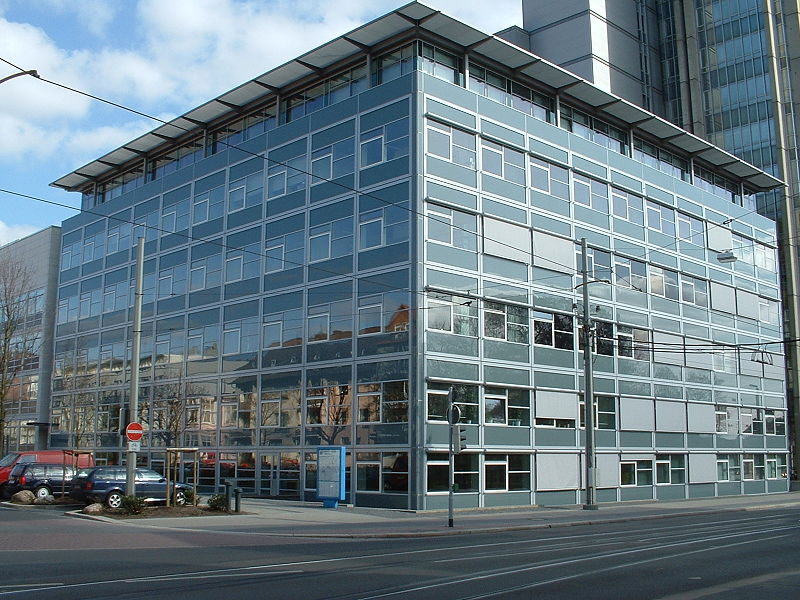
\includegraphics{infozentrum.jpg}}
\titlegraphic[scaled]{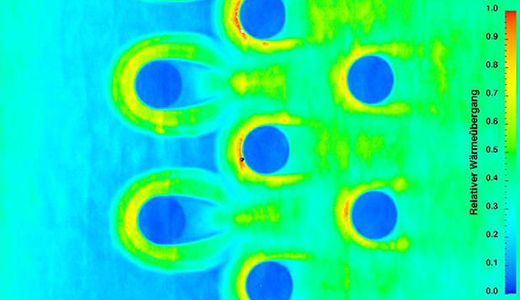
\includegraphics{Titelbild}}

% Logo, dass auf Titelseiten oben rechts und auf Inthaltsseiten unten rechts
% dargestellt wird. Es wird jeweils automatisch skliert
\logo{
\includegraphics{ift_4C.pdf}}
%\logo{Institut für Unkreativität\\und Schreibschwäche}

\begin{document}

\begin{frame}[plain]
\titlepage
\end{frame}

\begin{frame}[plain]
\centering
\textbf{{\huge Motivation}}
\end{frame}


\begin{frame}{Inhalt}
\begin{itemize}
\item {{\Large \textbf{Systemtheorie} }\\  Anwendungsmöglichkeiten für technische Systeme\vspace{0.3cm}}
\item {{\Large \textbf{Masterarbeit} }\\  Reglerstrukturen für Kälteprozesse mit dem Kältemittel $CO_2$\vspace{0.3cm}} 
\item {{\Large \textbf{Fazit} }} 
\end{itemize}
\end{frame}

\section{Systemtheorie}

\begin{frame}{Aufgabenbereiche}

\begin{exampleblock}{}
	\centering
	\textbf{ Technisches System}
\end{exampleblock}

  \begin{columns}[onlytextwidth]
    \column{0.45\textwidth}
	\begin{alertblock}{Reglerauslegung}
		\begin{itemize}
			\item Modell - \textit{einfach}
			\item Auslegungsmethoden
			\item Reglerstruktur
		\end{itemize}
	\end{alertblock}
    \column{0.45\textwidth}
	\begin{block}{Informationsgewinn}
		\begin{itemize}
			%\item Messung
			\item Modell - \textit{kompliziert}
			\item Datenverarbeitung
			\item Dynamik
		\end{itemize}
	\end{block}
  \end{columns}

\end{frame}

\begin{frame}{Informationsgewinn}
\begin{columns}[onlytextwidth]
    \column{0.45\textwidth}
	\begin{alertblock}{Vorraussetzungen}
		\begin{itemize}
			\item Messbarkeit
			\item Messdaten
			\item Parameterdaten
			\item Modell
		\end{itemize}
	\end{alertblock}
    \column{0.45\textwidth}
	%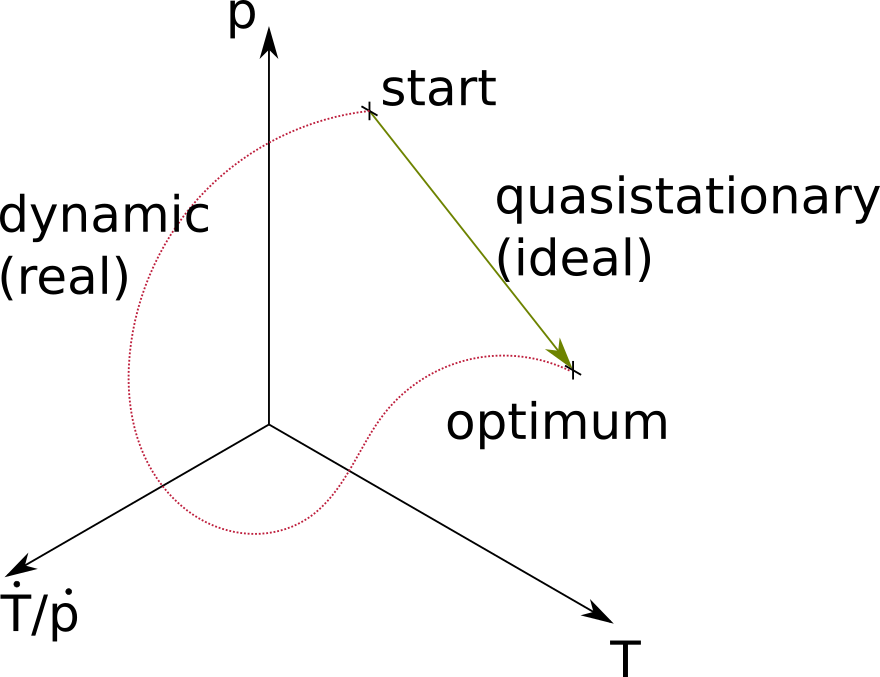
\includegraphics[width=\textwidth]{Trajektorie}
	\begin{block}{Vorteile}
		\begin{itemize}
			\item Komplexere Regler
			\item Data-Fusion
			\item Fehleranalyse
			\item Prozessbewertung
		\end{itemize}
	\end{block}
  \end{columns}

%\begin{columns}[onlytextwidth]
  %  \column{0.45\textwidth}
	%\begin{block}{Vorteile}
	%	\begin{itemize}
	%		\item Komplexere Regler
	%		\item Data-Fusion
	%		\item Fehleranalyse
	%		\item Prozessbewertung
	%	\end{itemize}
	%\end{block}
    %\column{0.45\textwidth}
	%\begin{exampleblock}{Vorteile}
	%	\begin{itemize}
	%		\item Flachheitsbasierte Regler
	%		\item Invertierende Regler
	%		\item Beobachter Entwürfe
	%	\end{itemize}
	%\end{exampleblock}
  %\end{columns}
\end{frame}

\begin{frame}{Anwendungsbeispiele}
\end{frame}

\begin{frame}{Reglerauslegung}
\centering
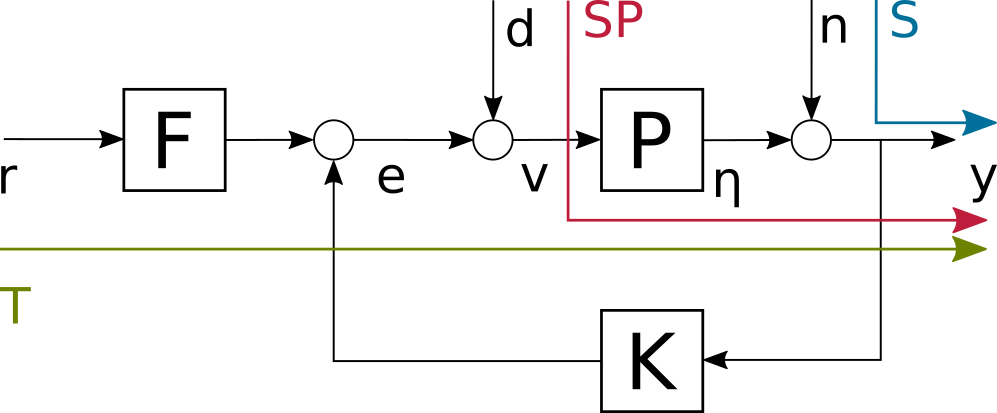
\includegraphics[width = 0.7\textwidth]{Reglerauslegung}
\begin{columns}[onlytextwidth]
    \column{0.45\textwidth}
	\begin{exampleblock}{Ziele}
		\begin{itemize}
			\item Stabilität
			\item (Statische) Sollwertfolge
			\item Performance
			\item Robustheit
		\end{itemize}
	\end{exampleblock}
    \column{0.45\textwidth}
	\begin{alertblock}{Probleme}
		\begin{itemize}
			\item \textbf{Information} ist begrenzt
			\item \textbf{Priorisierung} notwendig
		\end{itemize}
	\end{alertblock}
  \end{columns}

\end{frame}

\section{Masterarbeit - Reglerauslegung für Kälteprozesse}

\begin{frame}{Masterarbeit}
\begin{columns}[onlytextwidth]
    \column{0.45\textwidth}
\centering
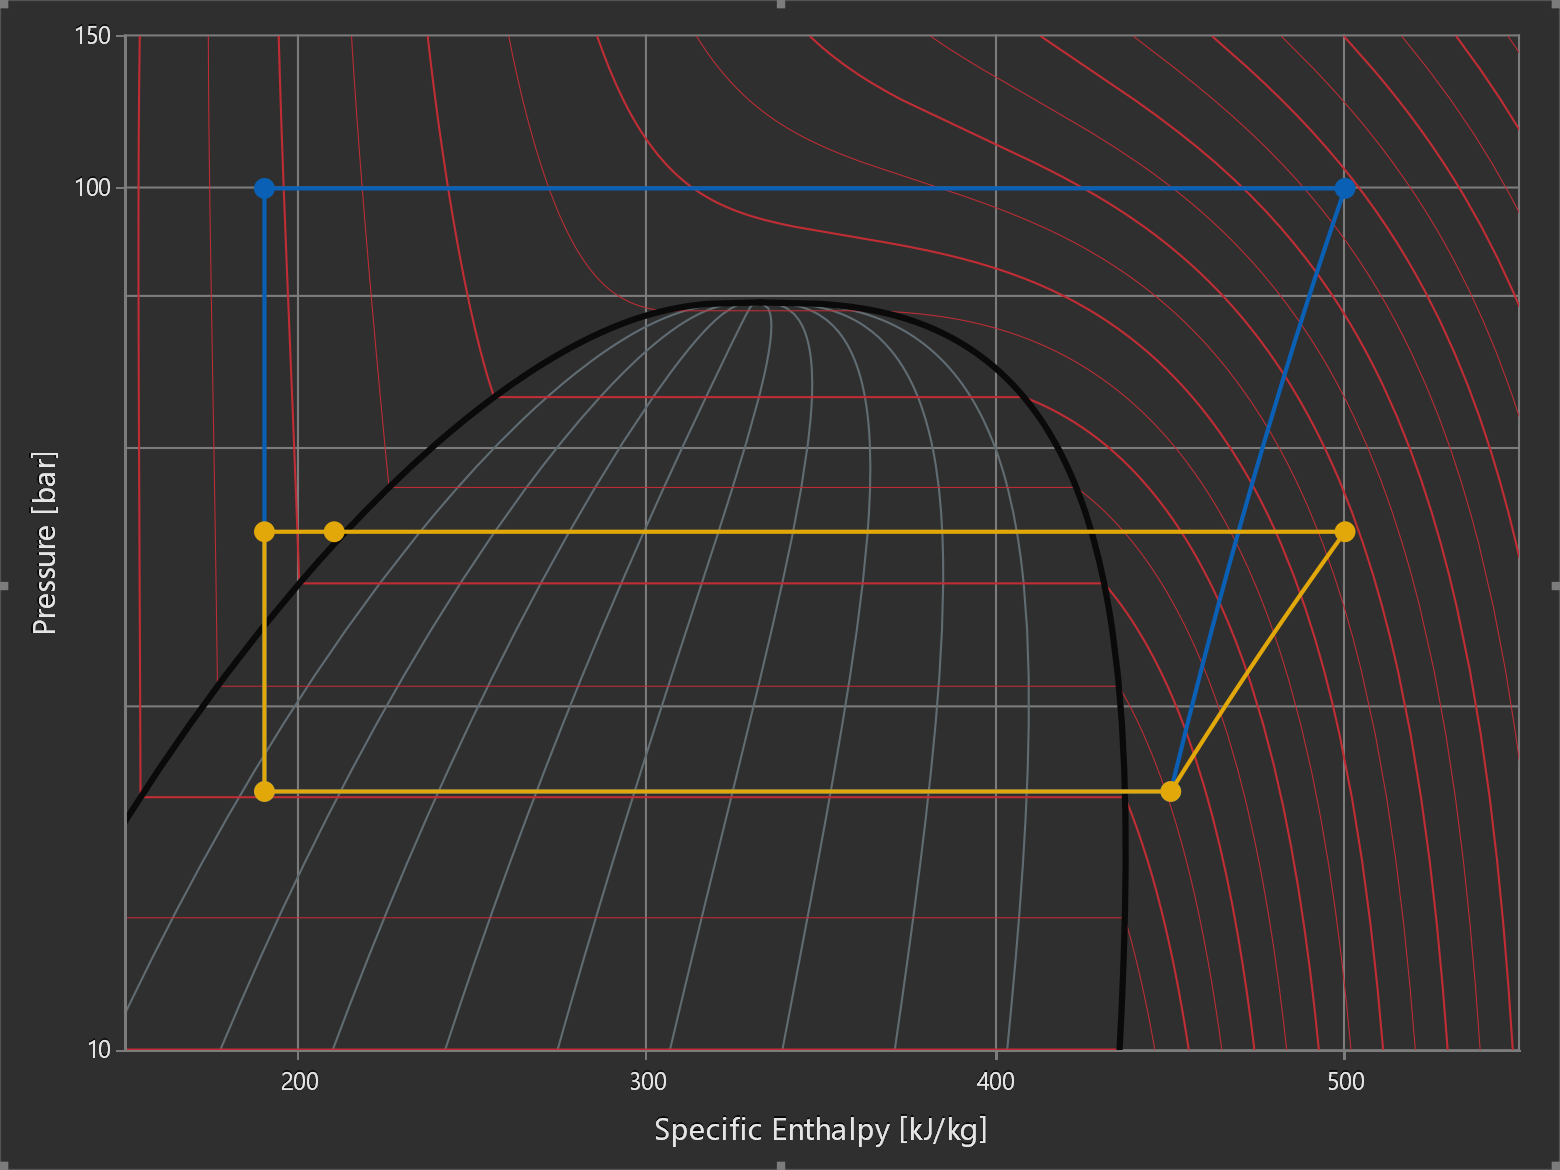
\includegraphics[width=\textwidth]{Prozess}
    \column{0.45\textwidth}
\begin{alertblock}{Aufgabe}
		\textbf{Autotuning} von \textbf{adaptiven},\textbf{dezentralen} Regelstrukturen.
	\end{alertblock}
	\begin{exampleblock}{Randbedingungen}
		\begin{itemize}
			\item Modell variiert stark
			\item Modell hochparametriert
			\item Reglerstruktur starr
			\item Reglerstruktur niedrig parametriert
		\end{itemize}
	\end{exampleblock}
  \end{columns}
\end{frame}

\begin{frame}{Ersatzmodell}
\centering
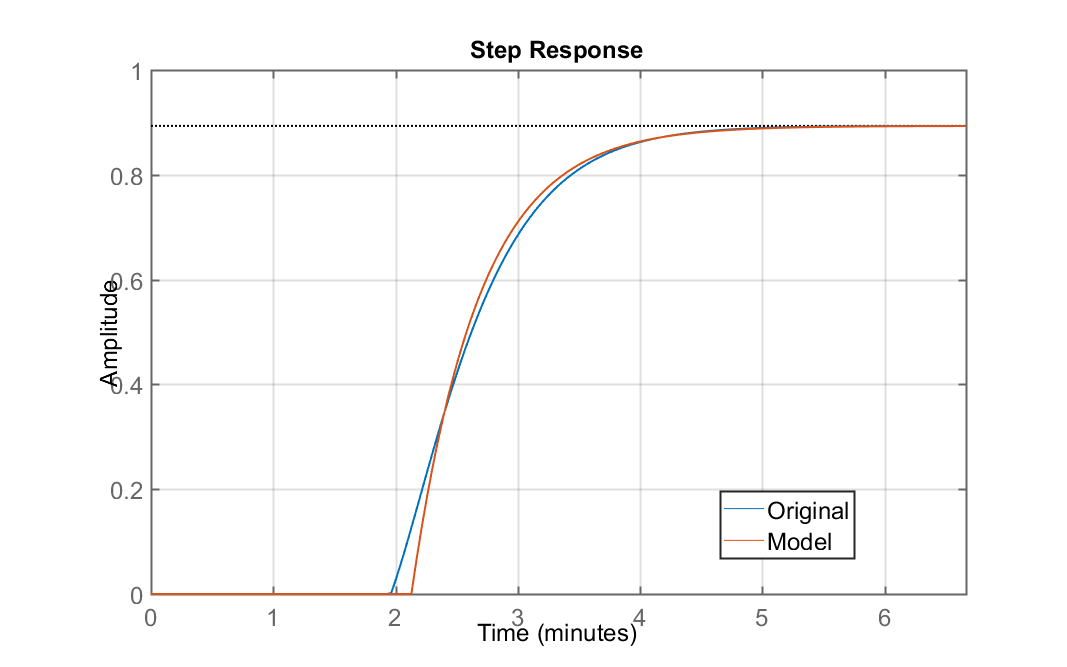
\includegraphics[width=\textwidth]{FOTD}
\end{frame}

\begin{frame}{Querkopplungen}
\begin{columns}[onlytextwidth]
    \column{0.45\textwidth}
	\begin{exampleblock}{Kopplungen}
		\textbf{Kopplungen} sind bekannt und können \textbf{minimiert} werden.
	\end{exampleblock}
	\begin{alertblock}{Nachteile}
		\textbf{Verlust} der nominellen \textbf{Performance} der Hauptkopplungen.
	\end{alertblock}
    \column{0.45\textwidth}
	\centering
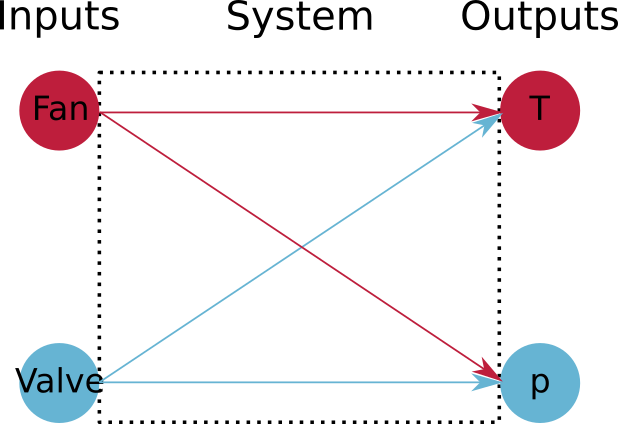
\includegraphics[width = \textwidth]{Querkopplungen}
  \end{columns}
\end{frame}

\begin{frame}{Beispiele - Performance}
\centering
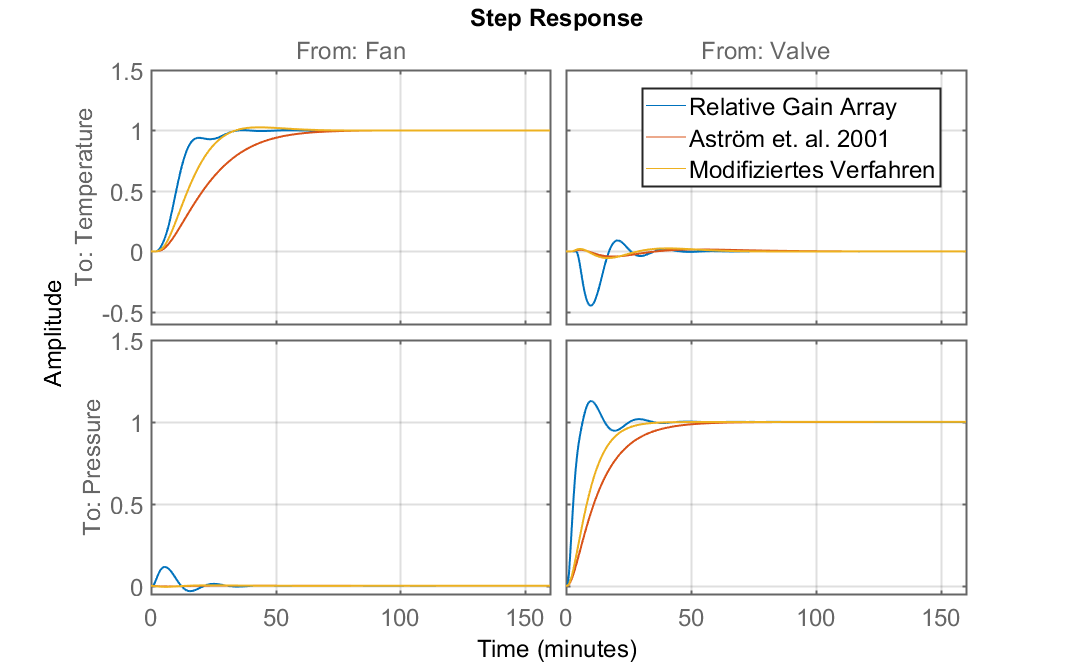
\includegraphics[width=\textwidth]{Stepresponse}
\end{frame}


\begin{frame}{Beispiele - Robustheit}
\centering
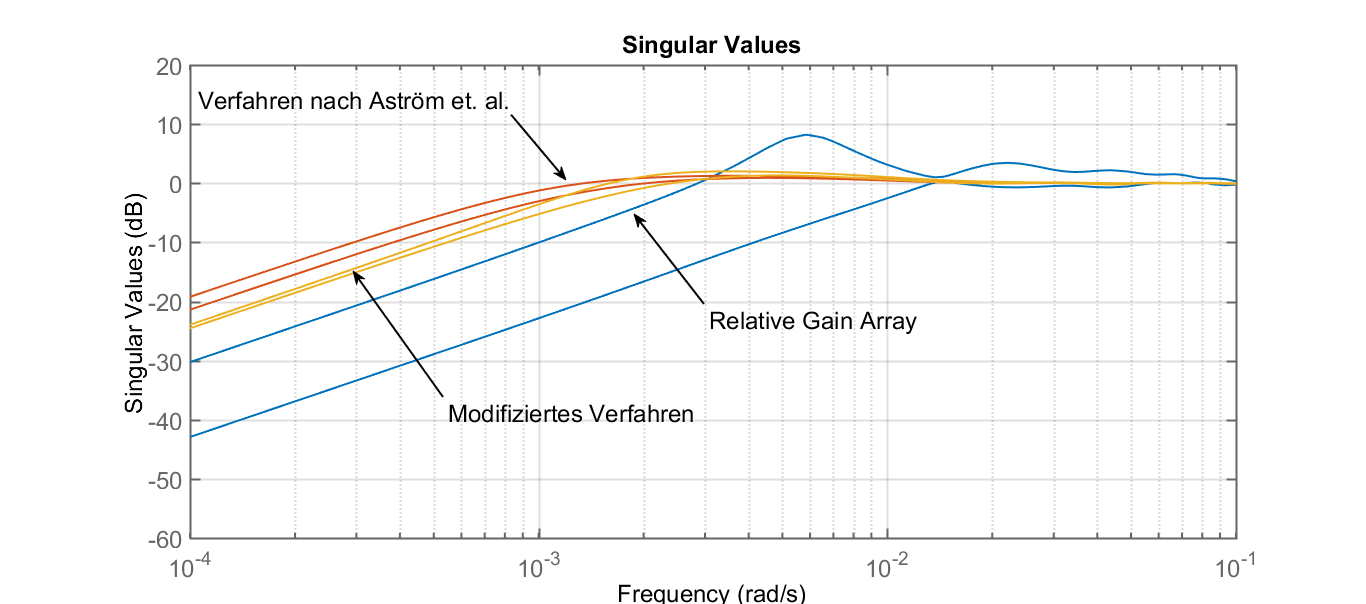
\includegraphics[width=\textwidth]{SVD}
\end{frame}

\section{Fazit}

\begin{frame}[highlight]{Perspektiven}
\begin{alertblock}{Reglerauslegung}
Einfache \textbf{Reglerauslegung} ist bereits bei einem stark \textbf{vereinfachten Modell} möglich.
\end{alertblock}
\begin{alertblock}{Performance}
\textbf{Optimale Performance} ist bei einem stark \textbf{vereinfachten Modell} für \textbf{nicht möglich}.
\end{alertblock}
\end{frame}


\begin{frame}[highlight]{Perspektiven}
\begin{block}{Systemtheorie}
\textbf{Informationsgehalt} und \textbf{-güte} kann durch \textbf{Systemtheorie} gesteigert werden.
\end{block}
\begin{block}{Systemdiagnose}
\textbf{Systemdiagnose} ist ausschließlich durch \textbf{hohe Modellgüte} sicher erreichbar.
\end{block}
\end{frame}


\begin{frame}{Abschluss}
\centering
\textbf{{\huge Fragen?}} \pause \\ \textbf{{\huge Vielen Dank für Ihre Aufmerksamkeit!}}
\end{frame}

\end{document}
